\documentclass{article}
\usepackage{amsmath, sfmath, multicol, tkz-euclide, array, enumerate, tcolorbox, tabularray, tipa}
\renewcommand{\familydefault}{\sfdefault}
\setlength{\parindent}{0cm}
\pagestyle{empty}
\usepackage[left=1in, top=0.5in, right=1in, bottom=0.5in]{geometry}
\tikzset{>=stealth, label style/.append style={font=\footnotesize}}
\tcbset{colback=white}

\newcounter{example}[section]
\newenvironment{example}[1][]{\refstepcounter{example}\par\medskip
   {\color{red}\textbf{Example~\theexample. #1}}}{\medskip}

\newcommand{\arc}[1]{%
    \setbox9=\hbox{#1}%
    \ooalign{\resizebox{\wd9}{\height}{\texttoptiebar{\phantom{A}}}\cr#1}}

\begin{document}

\section*{Angle Measure and Segment Length in Circles}

\begin{tcolorbox}[colframe=orange!70!white, coltitle=black, title=\textbf{Today I Can}]
\begin{enumerate}
    \item Find measures of angles formed by chords, secants, and tangents.
    \item Find the lengths of segments associated with circles.
\end{enumerate}
\end{tcolorbox}
\smallskip 

\begin{example}
Find the measure of the arc or angle indicated.
\begin{multicols}{2}
\begin{enumerate}[(a)]
    \item $m\arc{\textit{PR}}$
    \item $m\angle VTU$
\end{enumerate}
\end{multicols}
\begin{minipage}{0.5\textwidth}
    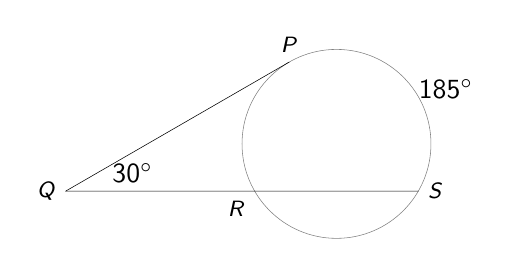
\begin{tikzpicture}[scale=0.8]
        \tkzDefPoints{0/0/O}
        \tkzDefShiftPoint[O](120:1.5){P}
        \tkzDrawCircle(O,P)
        \tkzLabelPoints[above](P)
        \tkzDefShiftPoint[O](-30:1.5){S}
        \tkzDefLine[orthogonal = through P](O,P)
        \tkzGetPoint{h}       
        \tkzLabelPoints[right](S)
        \tkzDefShiftPoint[S](180:6){a}
        \tkzInterLL(S,a)(P,h)
        \tkzGetPoint{Q}
        \tkzLabelPoints[left](Q)
        \tkzDrawSegments(P,Q S,Q)
        \tkzDefShiftPoint[O](210:1.5){R}
        \tkzLabelPoints[below left](R)
        \tkzLabelAngle[pos=1.1](S,Q,P){$30^\circ$}
        \tkzLabelAngle[pos=6.25](S,Q,P){$185^\circ$}
    \end{tikzpicture}
\end{minipage}
\begin{minipage}{0.4\textwidth}
    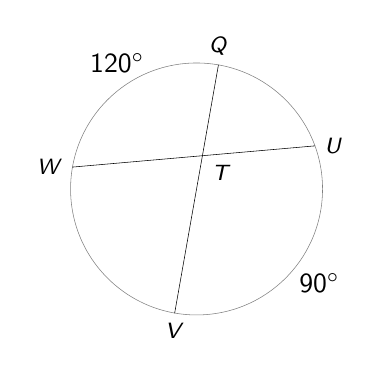
\begin{tikzpicture}[scale=0.8]
        \tkzDefPoints{0/0/O}
        \tkzDefShiftPoint[O](80:2){Q}
        \tkzDrawCircle(O,Q)
        \tkzLabelPoints[above](Q)
        \tkzDefShiftPoint[O](20:2){U}
        \tkzDefShiftPoint[O](170:2){W}
        \tkzDefShiftPoint[O](260:2){V}
        \tkzLabelPoints[right](U)
        \tkzLabelPoints[left](W)
        \tkzLabelPoints[below](V)
        \tkzDrawSegments(Q,V U,W)
        \tkzInterLL(Q,V)(U,W)
        \tkzGetPoint{T}
        \tkzLabelPoints[below right](T)
        \tkzLabelAngle[pos=-2.75](Q,T,W){$90^\circ$}
        \tkzLabelAngle[pos=2](Q,T,W){$120^\circ$}
    \end{tikzpicture}
\end{minipage}
\end{example}

\vspace{1in} 

\begin{example}
Solve for $x$ in each.
\begin{multicols}{2}
    \begin{enumerate}[(a)]
        \item \mbox \newline 
        \item \mbox \newline 
    \end{enumerate}
\end{multicols}
\begin{minipage}{0.5\textwidth}
    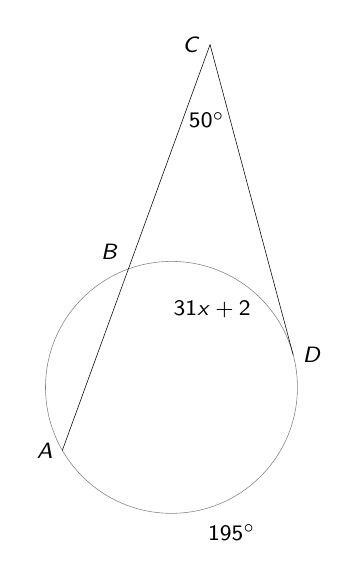
\begin{tikzpicture}[scale=0.8]
        \tkzDefPoints{0/0/O}
        \tkzDefShiftPoint[O](15:2){D}
        \tkzDrawCircle(O,D)
        \tkzLabelPoints[right](D)
        \tkzDefLine[orthogonal = through D](O,D)
        % \tkzTangent[at=D](O)
        \tkzGetPoint{h}
        \tkzDefShiftPoint[O](110:2){B}
        \tkzLabelPoints[above left](B)
        \tkzDefShiftPoint[O](210:2){A}
        \tkzInterLL(A,B)(D,h)
        \tkzGetPoint{C}
        \tkzLabelPoints[left](A, C)
        \tkzDrawSegments(C,A C,D)
        \tkzLabelAngle[pos=2.5](A,O,D){\footnotesize $195^\circ$}
        \tkzLabelAngle[pos=1.4](D,O,B){\footnotesize $31x+2$}
        \tkzLabelAngle[pos=1.2](B,C,D){\footnotesize $50^\circ$}
    \end{tikzpicture}
\end{minipage}
\begin{minipage}{0.4\textwidth}
    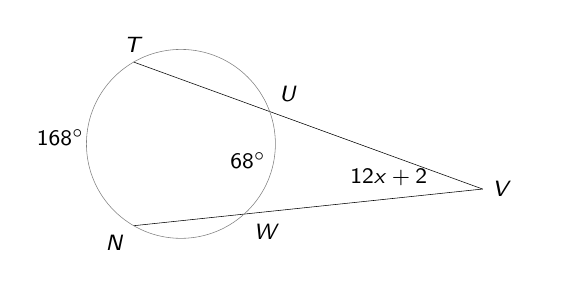
\begin{tikzpicture}[scale=0.8]
        \tkzDefPoints{0/0/O}
        \tkzDefShiftPoint[O](20:1.5){U}
        \tkzDefShiftPoint[O](-48:1.5){W}
        \tkzDefShiftPoint[O](120:1.5){T}
        \tkzDefShiftPoint[O](240:1.5){N}
        \tkzInterLL(T,U)(N,W)
        \tkzGetPoint{V}
        \tkzDrawSegments(T,V N,V)
        \tkzDrawCircle(O,T)
        \tkzLabelAngle[pos=-6.75](N,V,T){\footnotesize $168^\circ$}
        \tkzLabelAngle[pos=-3.75](N,V,T){\footnotesize $68^\circ$}
        \tkzLabelAngle[pos=-1.5](N,V,T){\footnotesize $12x+2$}
        \tkzLabelPoints[above](T)
        \tkzLabelPoints[above right](U)
        \tkzLabelPoints[right](V)
        \tkzLabelPoints[below right](W)
        \tkzLabelPoints[below left](N)
    \end{tikzpicture}
\end{minipage}

\vfill 
\newpage 

\begin{multicols}{2}
    \begin{enumerate}[(a)]  \setcounter{enumi}{2}
        \item \mbox \newline 
        \item \mbox \newline 
    \end{enumerate}
\end{multicols}
\begin{minipage}{0.5\textwidth}
    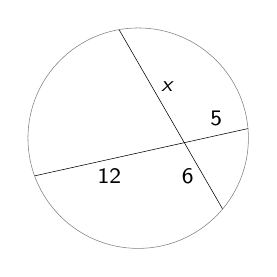
\begin{tikzpicture}[scale=0.8]
        \tkzDefPoints{0/0/O}
        \tkzDefShiftPoint[O](5:1.75){A}
        \tkzDefShiftPoint[O](-40:1.75){B}
        \tkzDefShiftPoint[O](100:1.75){C}
        \tkzDefShiftPoint[O](200:1.75){D}
        \tkzDrawSegments(A,D B,C)
        \tkzDrawCircle(O,C)
        \tkzInterLL(A,D)(B,C)
        \tkzGetPoint{E}
        \tkzLabelSegment[above](A,E){5}
        \tkzLabelSegment[left](B,E){6}
        \tkzLabelSegment[right](C,E){$x$}
        \tkzLabelSegment(D,E){12}
    \end{tikzpicture}
\end{minipage}
\begin{minipage}{0.4\textwidth}
    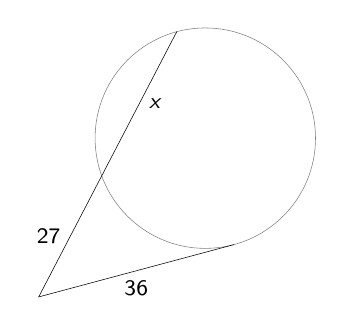
\begin{tikzpicture}[scale=0.8]
        \tkzDefPoints{0/0/O}
        \tkzDefShiftPoint[O](105:1.75){A}
        \tkzDefShiftPoint[O](200:1.75){B}
        \tkzDrawCircle(O,A)
        \tkzDefShiftPoint[O](285:1.75){C}
        \tkzDefLine[orthogonal = through C](O,C)
        \tkzGetPoint{h}
        \tkzInterLL(A,B)(C,h)
        \tkzGetPoint{e}
        \tkzDrawSegments(A,e C,e)
        \tkzLabelSegment[below](C,e){36}
        \tkzLabelSegment[left](e,B){27}
        \tkzLabelSegment[right](A,B){$x$}
    \end{tikzpicture}
\end{minipage}

\vfill 

\begin{enumerate}[(a)]  \setcounter{enumi}{4}
    \item \mbox \newline 
    
    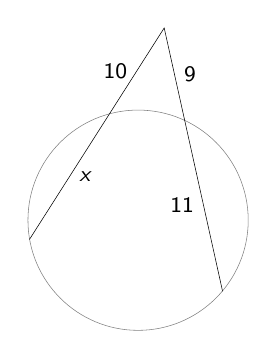
\begin{tikzpicture}[scale=0.8]
        \tkzDefPoints{0/0/O}
        \tkzDefShiftPoint[O](-40:1.75){E}
        \tkzDrawCircle(O,E)
        \tkzDefShiftPoint[O](65:1.75){C}
        \tkzDefShiftPoint[O](105:1.75){B}
        \tkzDefShiftPoint[O](190:1.75){D}
        \tkzInterLL(E,C)(D,B)
        \tkzGetPoint{A}
        \tkzDrawSegments(A,D A,E)
        \tkzLabelSegment[right](B,D){$x$}
        \tkzLabelSegment[right](A,C){9}
        \tkzLabelSegment[left](A,B){10}
        \tkzLabelSegment[left](C,E){11}
    \end{tikzpicture}
\end{enumerate}
\end{example}

\vfill 

\end{document}
